Every good design needs a diagram. This can be in the form of timing diagrams, block diagrams, class diagrams. Never over estimate your own ability to forget what you were doing or how you were approaching a design. Even with small designs I'm constantly scribbling on pieces of paper to straighten out exactly what I'm looking to implement. 

Many great tools exist for creating design diagrams, and you're welcome to use any of them for completing your design; however, I'll point you towards Mermaid Diagramming Markdown language as a great option for building powerful diagrams. 

While we cannot cover all the details of the setup. Here's an example diagram illustrating the functionality of a simple PWM module like the one provided in LAB 2.
\begin{verbatim}
    graph TB
    CNT["Counter 8-bits"]
    PWM["PWM Output"]
    CLK["CLK_IN"]
    DUT["DUTY"]
    MAX["MAX VALUE"]
    LESS([<])
    GRT([>])
  
        CLK -- "Increment" --> CNT
        CNT -->LESS
        DUT --->LESS
        LESS -->PWM
        MAX --->GRT
        CNT--> GRT
        GRT --"RESET"--> CNT
\end{verbatim}

The above code produces the following diagram:
\begin{figure} [H]
    \centering
    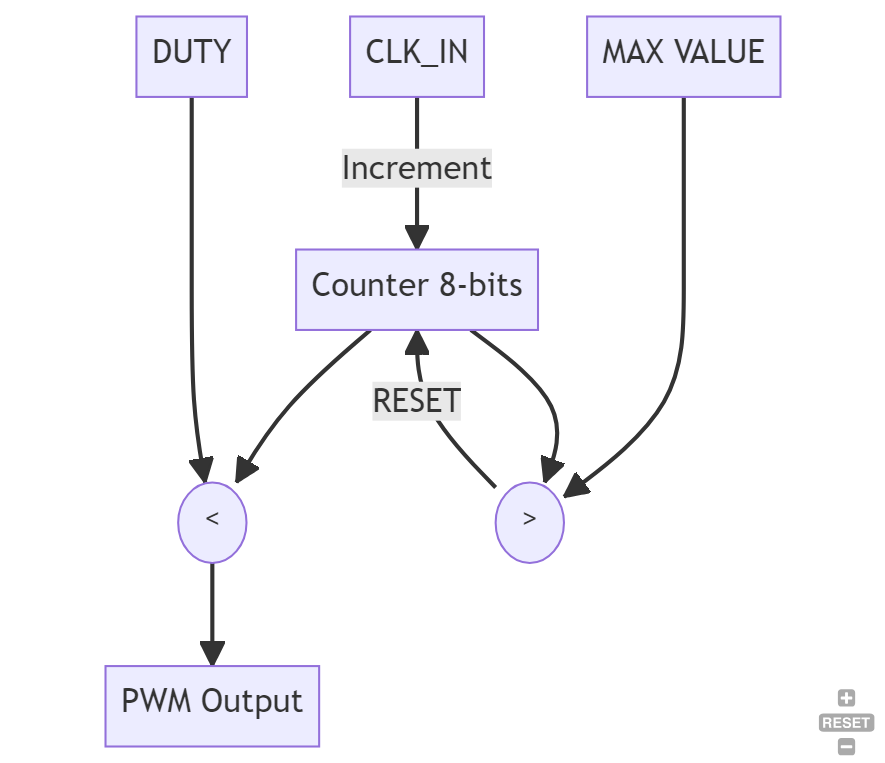
\includegraphics[width = 9cm]{Images/ProvidedPWM/PWM_block_diagram.png}
    \caption{PWM Block diagram generated with Mermaid Code}
    \label{fig:enter-label}
\end{figure}

If you would prefer to avoid hand drawing diagrams I recommend giving this system a try. It is freely available online at \url{https://mermaid.js.org/} and can be accessed without signing up. The provided design has been diagrammed below alongside the code.

\begin{verbatim}
    flowchart TD

clk["CLK"]
rst["RST"]
start_btn["STRT_BTN"]
stop_btn["STOP_BTN"]
inc_min["INC_MIN"]
inc_sec["INC_SEC"]
mod_sw["Mode Switch"]

sev_seg["Seven Segment"]
anode["Anode"]


blink_disp["blinking_display.sv"]
debounce["debounce.sv"]
display["display_driver.sv"]
one_s["one_second.sv"]


timer["timer.sv"]

clk --> one_s
rst --> one_s
one_hz["CLK_1Hz"]
one_k["CLK_1KHz"]
one_s --> one_hz
one_s --> one_k
one_k-->timer

an_in["anode"]
an_in --> blink_disp
clk --> blink_disp
rst --> blink_disp
one_hz --> blink_disp
blink_disp --> anode

clk --> display
rst --> display
min["Minutes"]
sec["Seconds"]
min --> double_dabble
sec --> double_dabble
seg_m ----> sev_seg
seg_m --> an_in

start_btn --> debounce
stop_btn --> debounce
inc_min --> debounce
inc_sec --> debounce
debounce --> timer
debounce --> timer
debounce --> timer
debounce --> timer
mod_sw --> timer
clk --> timer
rst --> timer
timer --> blink_disp

subgraph display
    bcd_binary["bcd_binary.sv"]
    
    double_dabble["double_dabble.sv"]
    sevenseg4ddriver["sevenseg4ddriver.sv"]

    double_dabble --> bcd_binary
    bcd_binary -->seg_m
    subgraph sevenseg4ddriver
        seg_m["segment_mux.sv"]
        pwm["pwm_module.sv"]
        pwm--> seg_m
    end
end

subgraph timer
    tim_c["time_counter.sv"]
end
timer -->sec
timer -->min

\end{verbatim}

\begin{figure}[H]
    \centering
    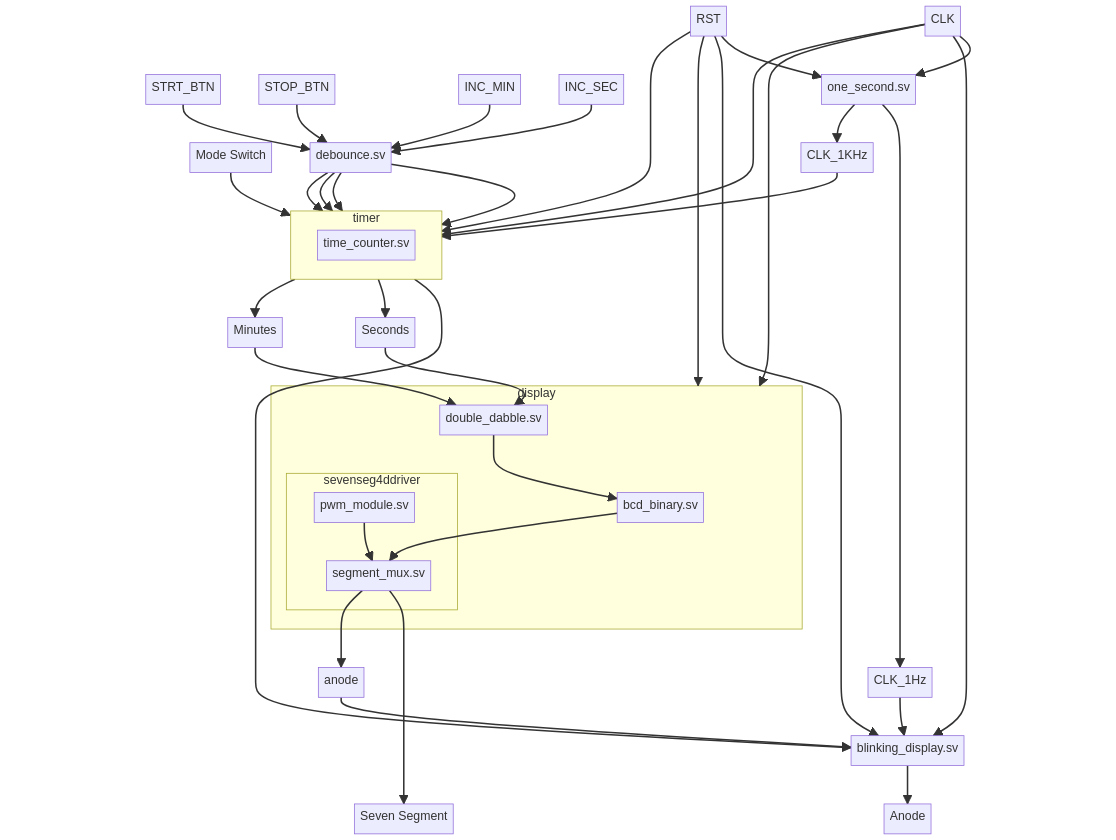
\includegraphics[width = \textwidth]{Images/SystemBlockDiagram.png}
    \caption{Timer System Diagram}
    \label{fig:Timer Diagram}
\end{figure}
I will note that this diagram is not perfect. It leaves out some of the finer details, like the active high versus active low reset, and duplicate instantiating of modules such as the debounce module. However, it shows sufficient details that if I am returning to this design in the future I will be able to work with and update the design appropriately without needing to read large portions of the document. 